\documentclass{beamer}
 
\usepackage[utf8]{inputenc}
\usepackage[english]{babel}
\usepackage{amsmath}
\usepackage{amsfonts}
\usepackage{amssymb}
\usepackage{graphicx} 
\usepackage{latexsym} 
\usepackage{listings}
\usepackage{xcolor}
\usepackage{soul}
\usepackage[T1]{fontenc}
\usepackage{amsthm}
\usepackage{mathtools}
\usepackage{setspace}
\usepackage{array,multirow,makecell}
\usepackage{geometry}
\usepackage{textcomp}
\usepackage{float}
\usepackage{bbold}
\usepackage{wrapfig}
\usepackage{textpos}

\rmfamily

\usetheme{Madrid}
%%\usecolortheme{beaver}



\title{LP 40 Confinement d'une particule et quantification de l'énergie}
\author{Naïmo Davier}
\institute{Université Paul sabatier}

 
\begin{document}
	
\begin{frame}
	\titlepage
\end{frame}

\addtocounter{framenumber}{-1}
\title{Quantification de l'énergie}

\begin{frame}
\frametitle{Potentiel effectif : potentiel central et moment cinétique}
\centerline{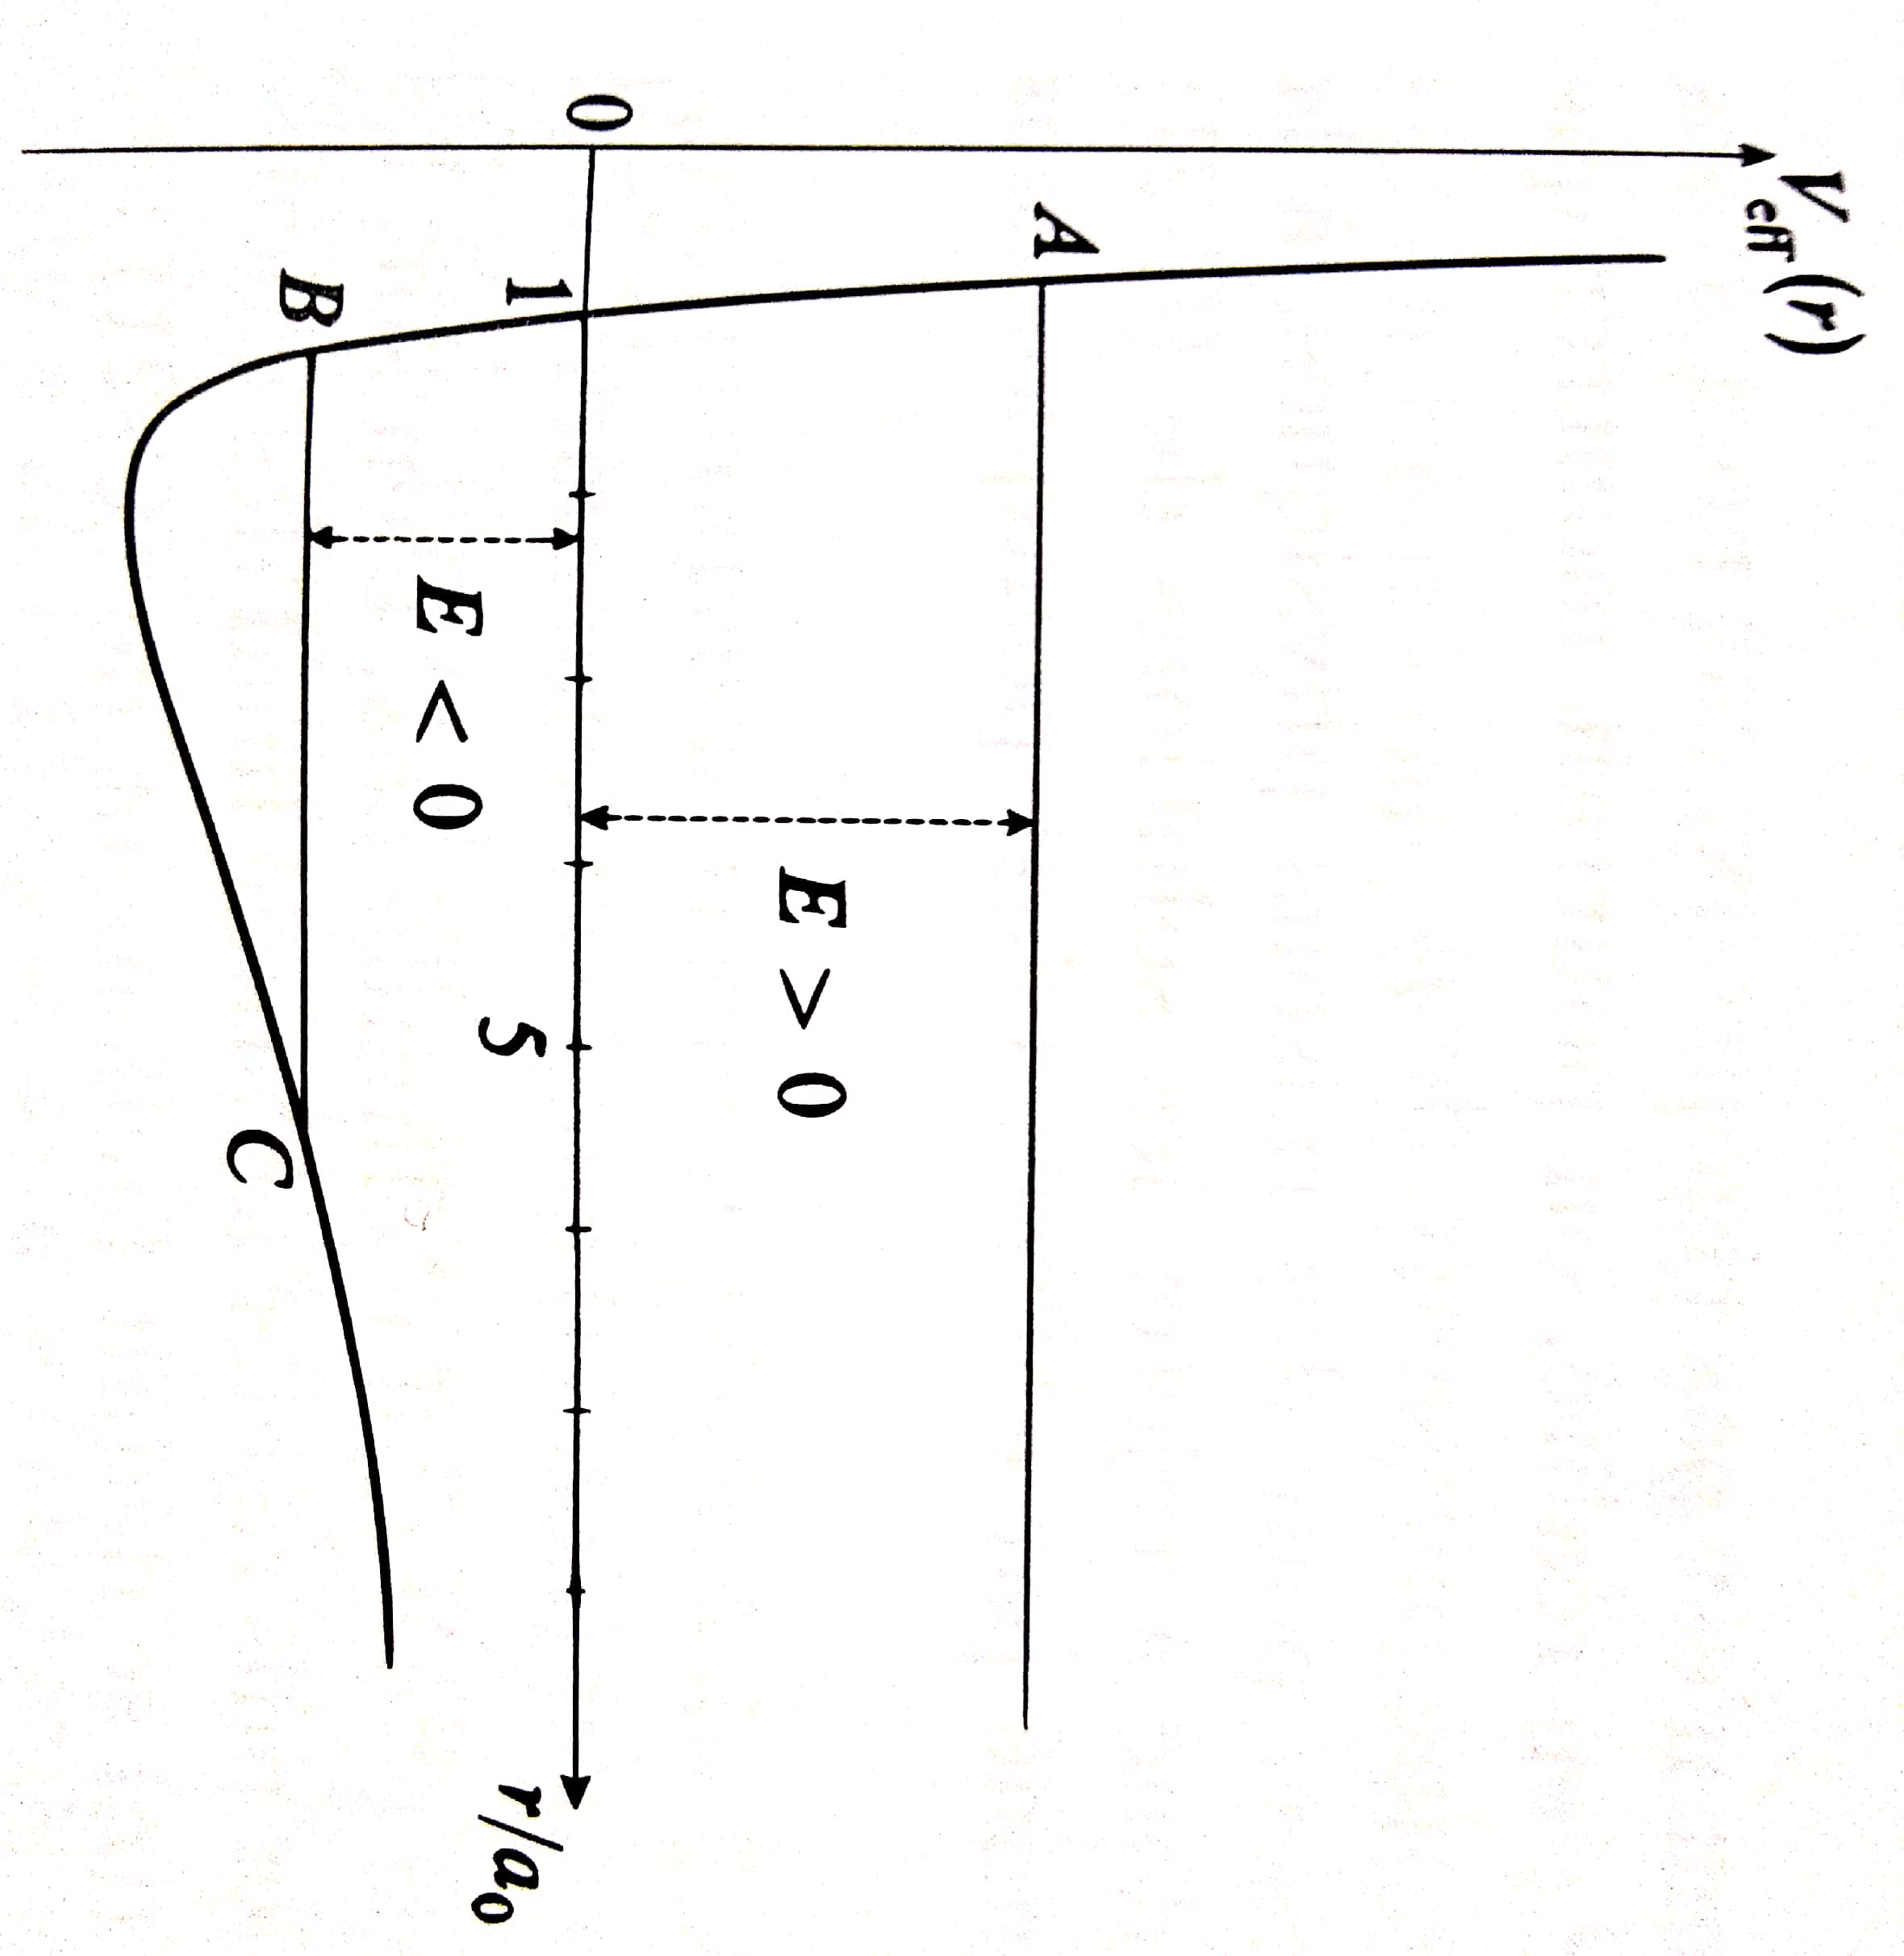
\includegraphics[width=8cm, angle=90]{potentiel}}
\end{frame}

\begin{frame}
\frametitle{Niveaux d'énergie}
\centerline{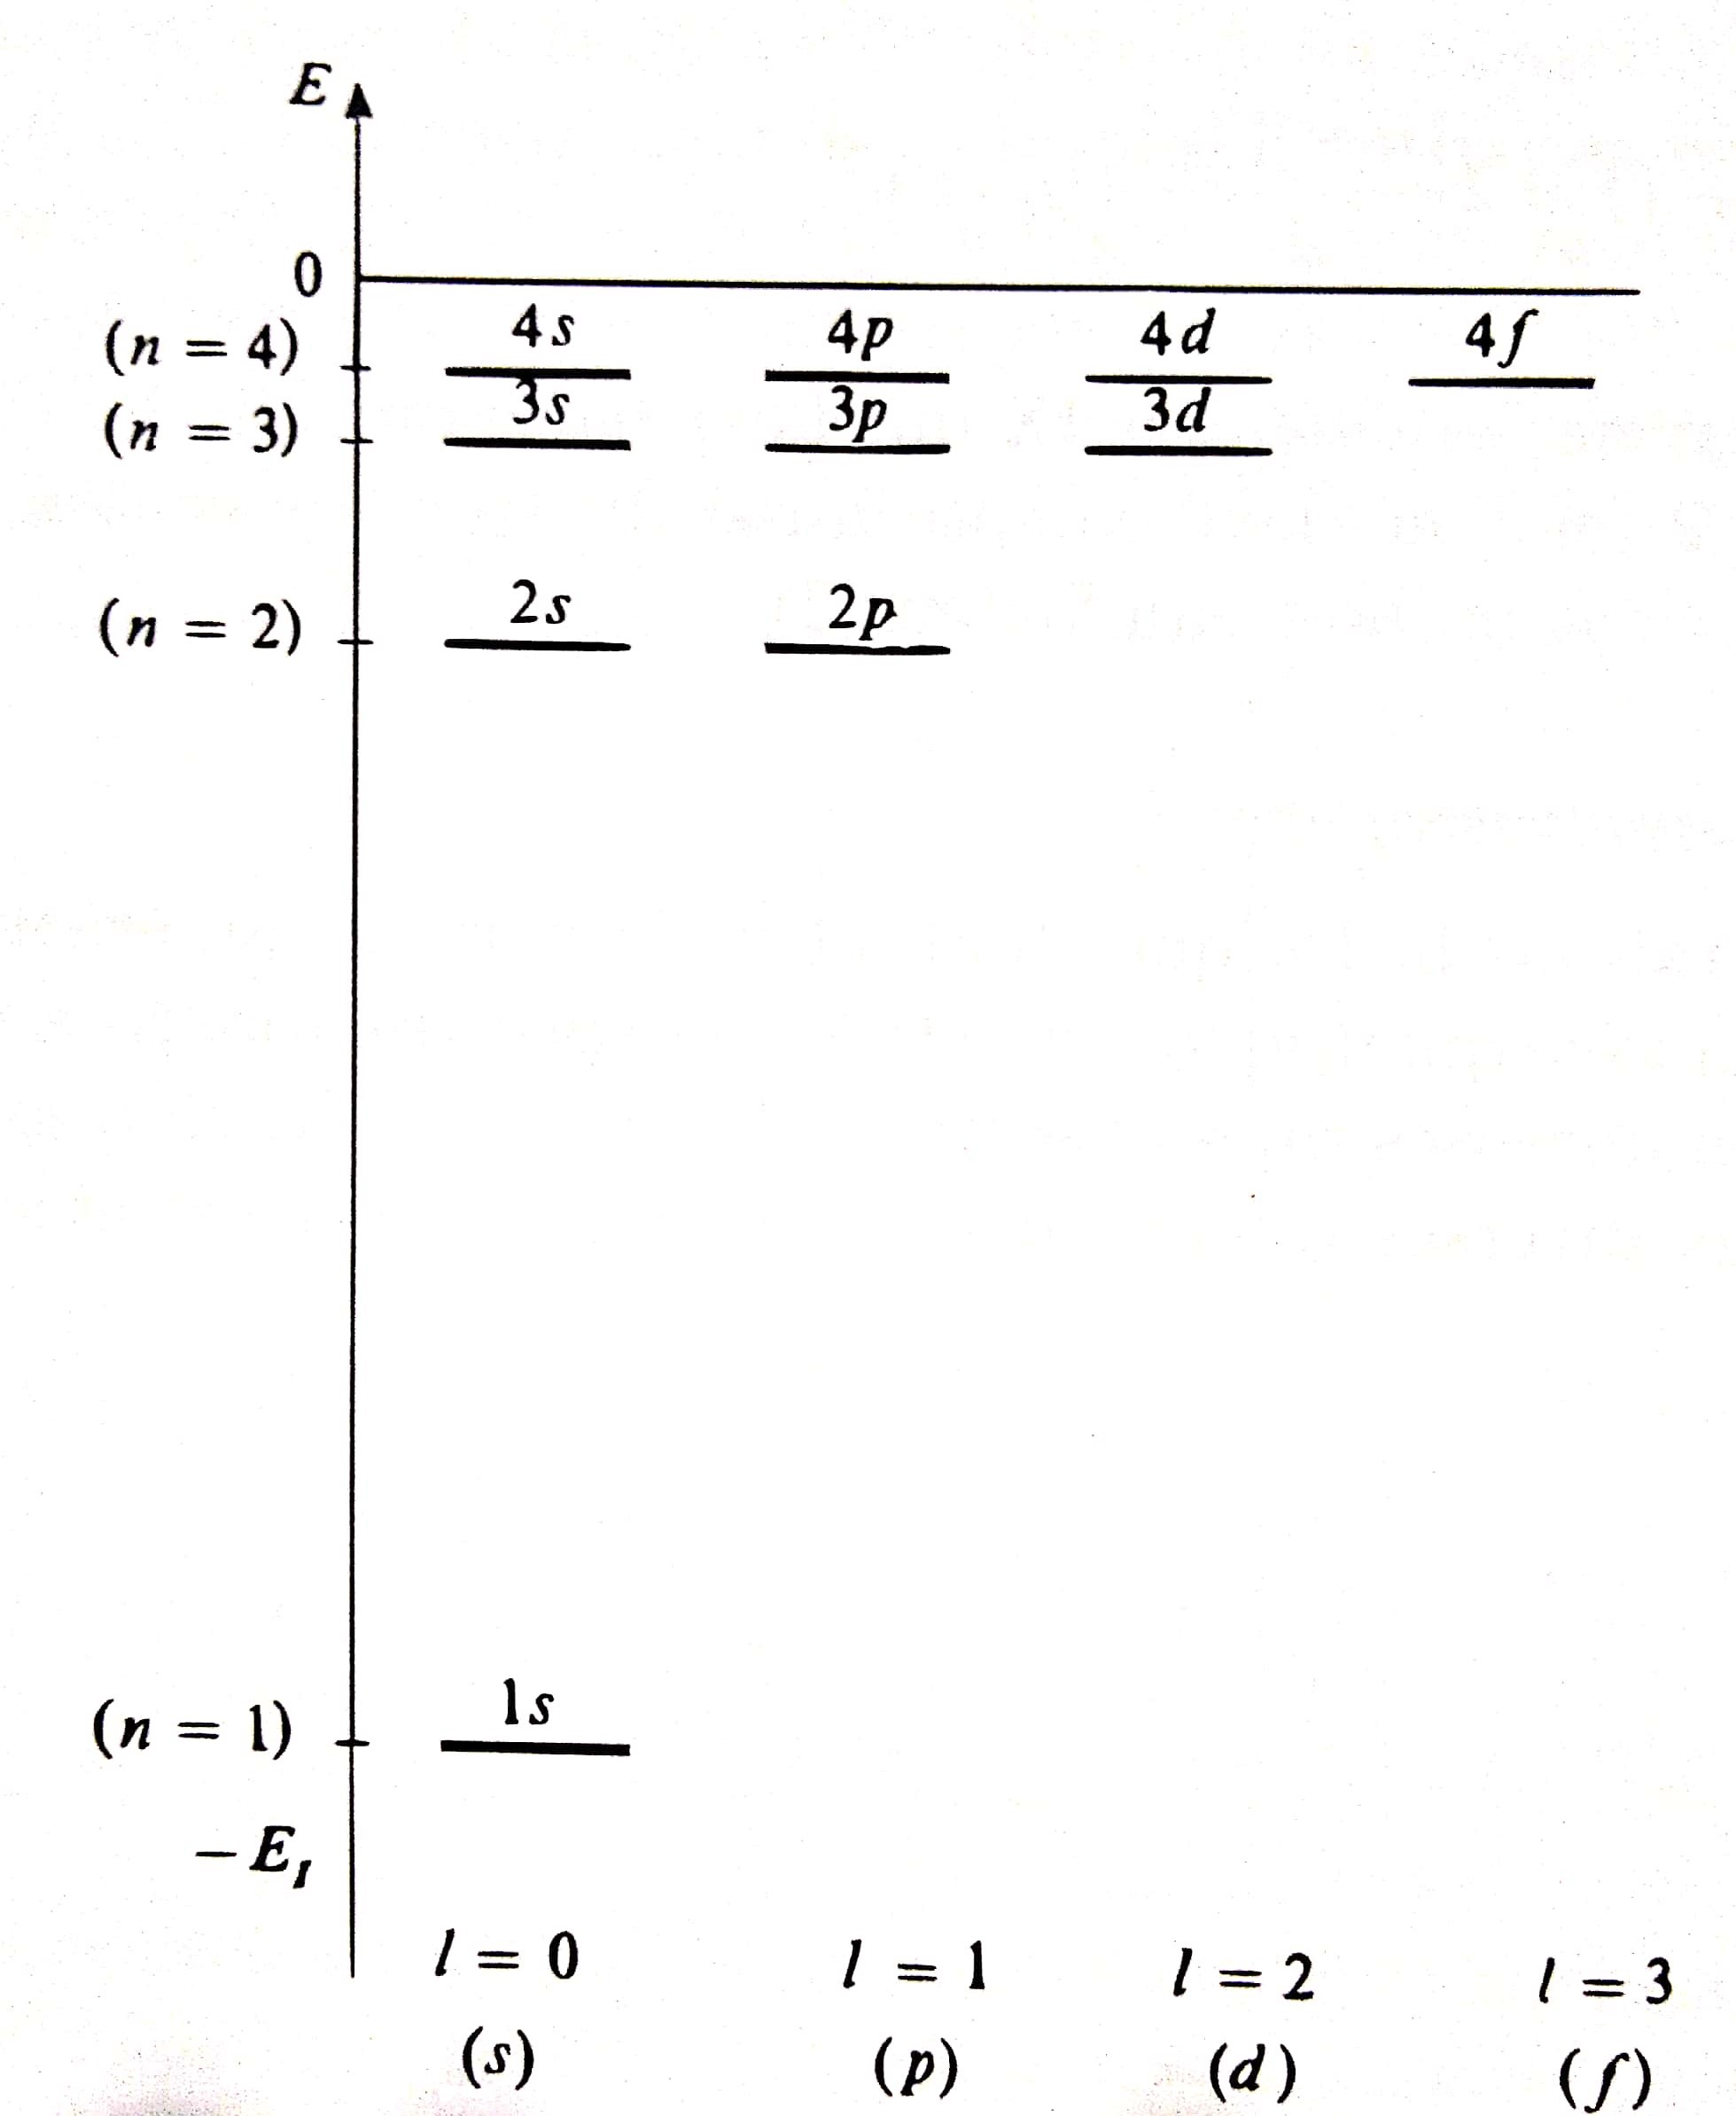
\includegraphics[width=6cm]{niveaux_energie}}
\end{frame}

\begin{frame}
\frametitle{Solutions et géométries}
\centerline{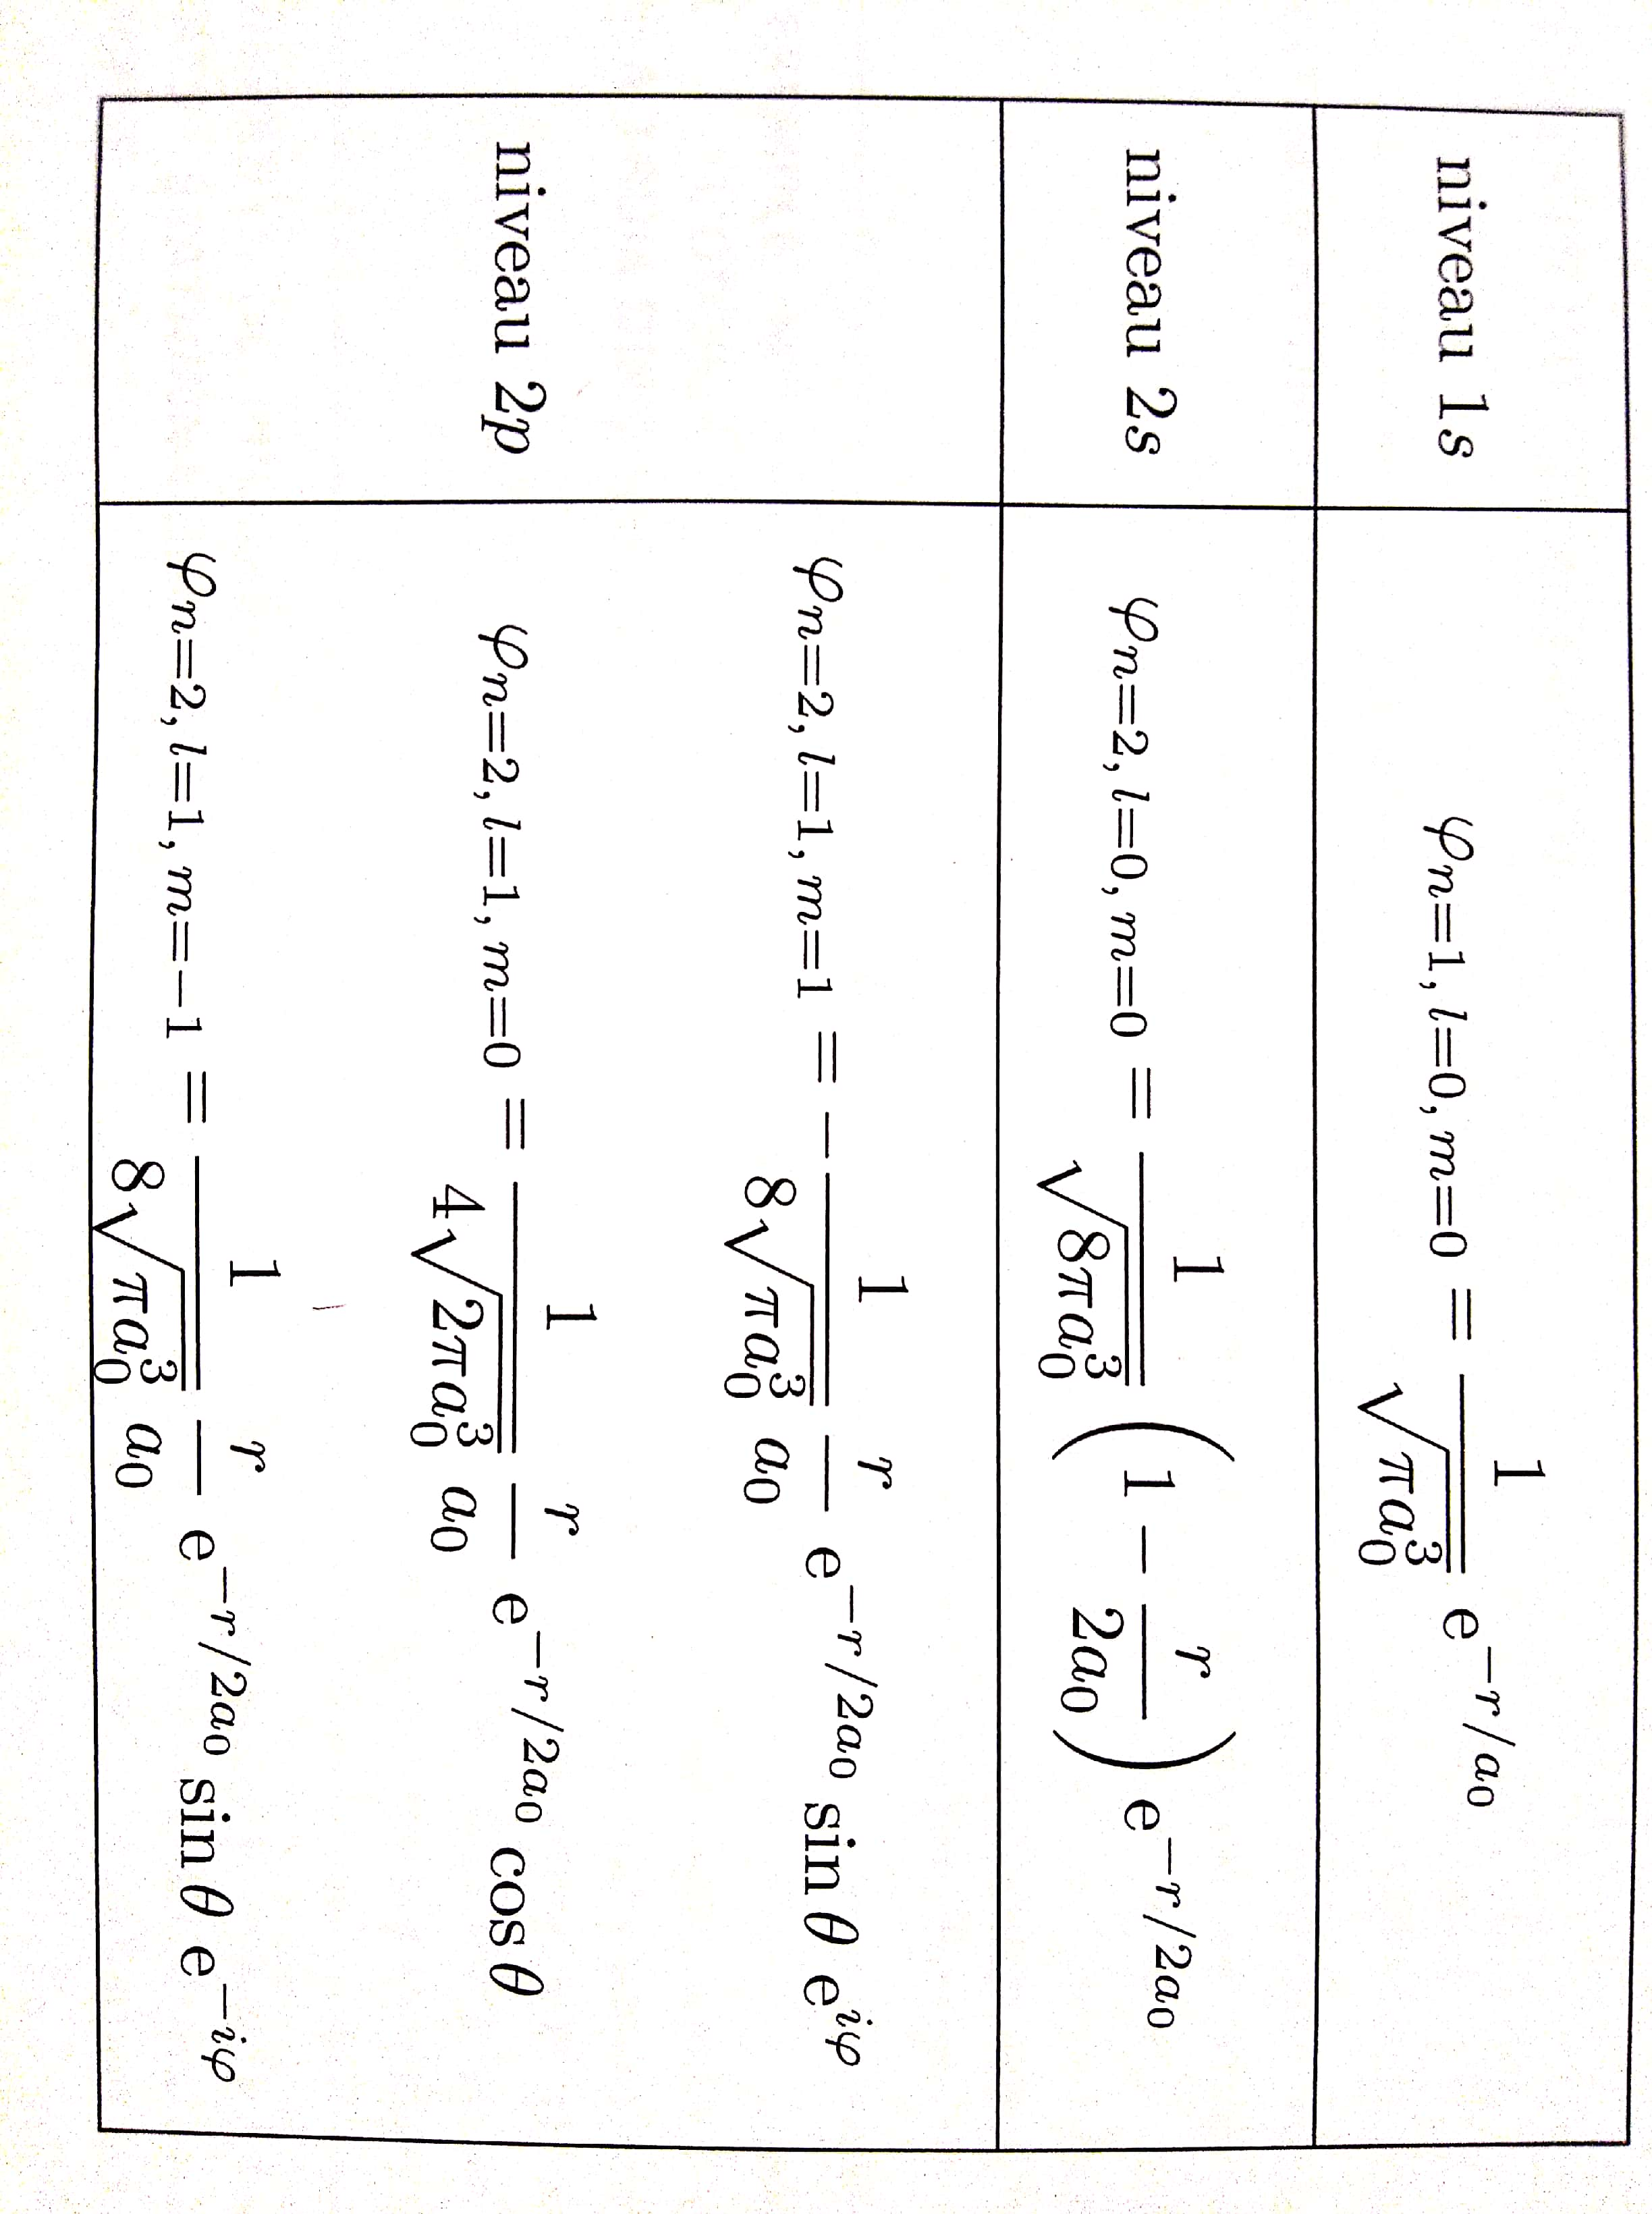
\includegraphics[width=5.5cm, angle=90]{phi(r)}
			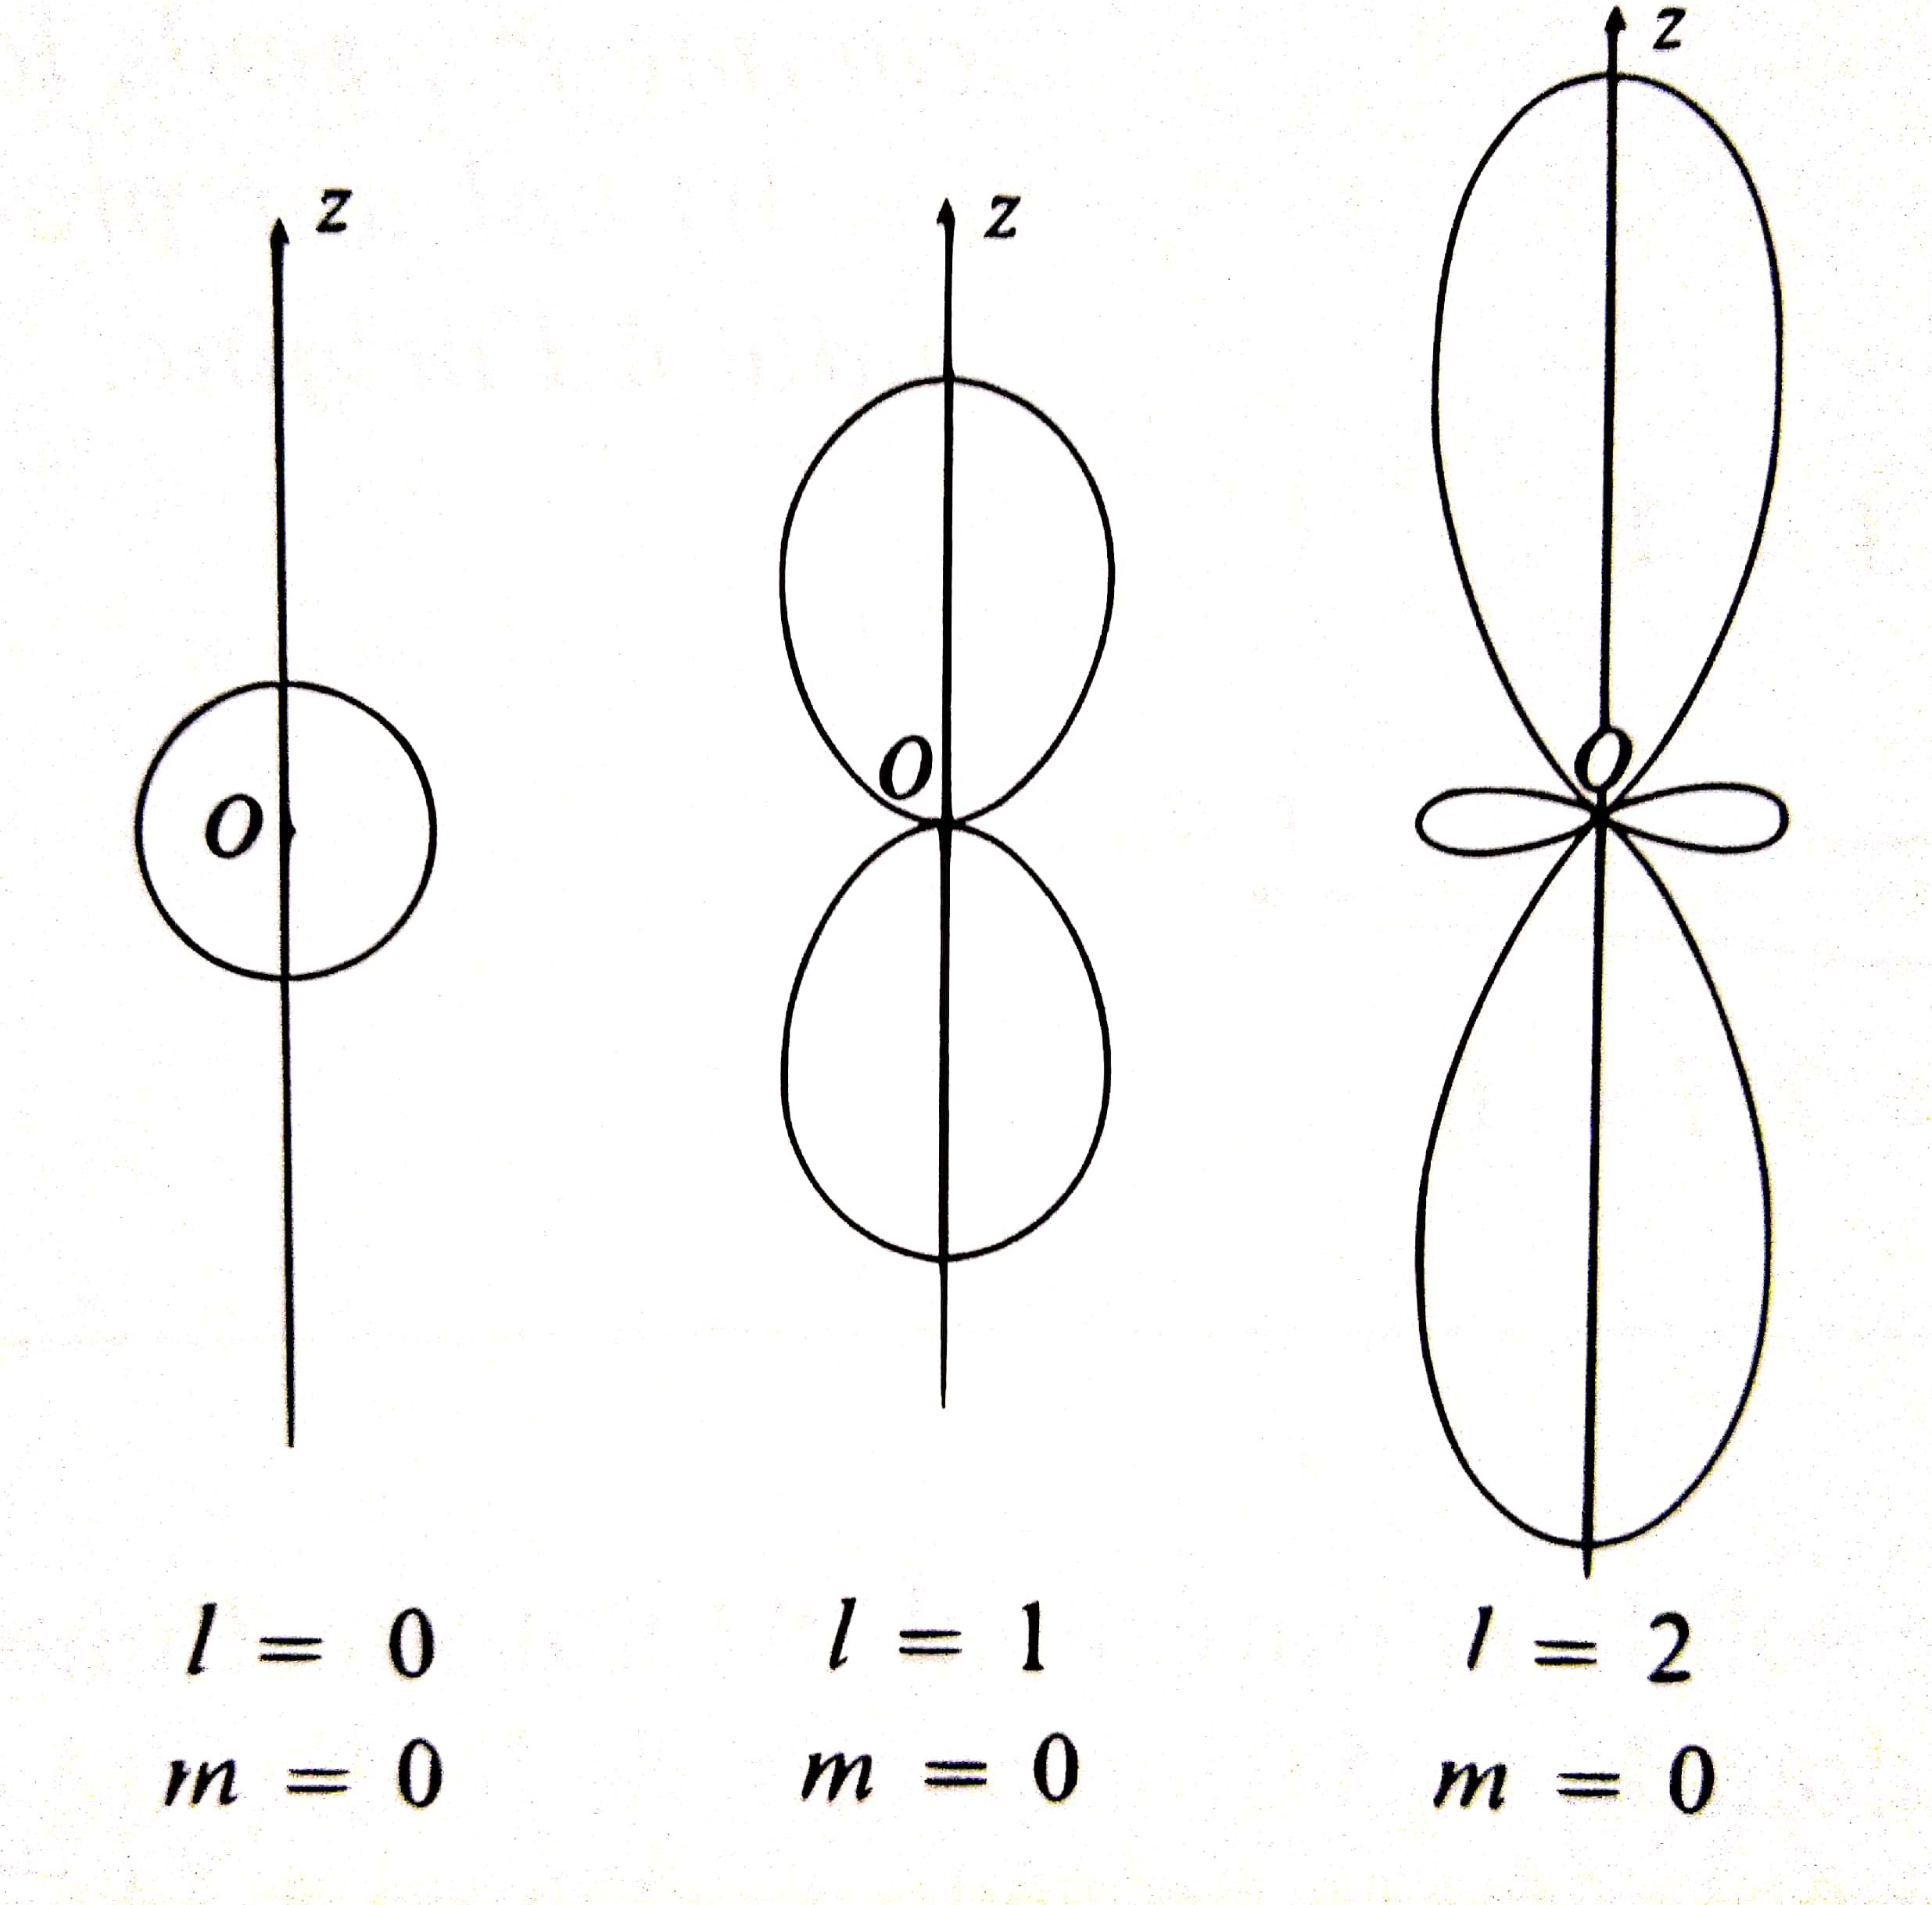
\includegraphics[width=5cm]{orbitales}}
\end{frame}

\end{document}